\appendix
\chapter{Appendix}

\section{OpenVINO Model Optimizer}
Model Optimizer is a python based tool which takes a pre-trained CNN model (.pb file) as its input and converts it to an intermediate representation consisting of a .xml file containing the network topology and a .bin file containing the layer weights. This makes the high level training frameworks such as Tensorflow and Caffe independent of the underlying hardware platforms. The steps to generate the IR are as follows:-

\begin{itemize}
    \item Download an available pre-trained CNN model. We have used the slim image classification library models in our project.
    \item The model is available as a single .ckpt file, for which the inference graph needs to be exported in the form of a .pb file.
    \item The model can now be frozen to give a single big .pb file which contains both the topology and the weights of the model.
    \item This frozen model can now be used to generate IR through the  command given in Code \ref{code:Model_opt}.
\end{itemize}

\begin{code}[!htb]
 \begin{minted}[fontsize=\small]{bash}
[user@fe-1 ~]$ python \  
/opt/intel/computer_vision_sdk_2018.5.455/deployment_tools/model_optimizer/mo_tf.py \ 
--input_model ./vgg_19_frozen.pb --input_shape [1,224,224,3] \
--mean_value [127.5,127.5,127.5] --scale 127.5

\end{minted}
\caption{Command to invoke Model Optimizer}
\label{code:Model_opt}
\end{code}

\section{Build Inference Engine Project on CC Frontend.}
\textbf{Software Requirements:}
\begin{itemize}
\item cmake 3.9 or higher
\item gcc 4.8 or higher
\end{itemize}
\textbf{Cloning the DLDT repository:}
We need to clone the open source Deep Learning Deployment Toolkit repository.

\begin{itemize}
\item execute the following command to clone the DLDT repository. \\* \raggedright\texttt{ git@git.uni-paderborn.de:cs-hit/pg-custonn2-2018-3rd-party/dldt.git}   
\item Once the DLDT repository is cloned, we need to clone a sub project \textbf{ade} into the project. Navigate to dldt dir and execute the command \\* \texttt{git submodule init} \\*  followed by \\* \texttt{git submodule update --recursive}. \\* 
\end{itemize}

\textbf{Build Steps:}

\begin{itemize}
\item Navigate to \\* \texttt{cd <dldt>/inference-engine}
\item Create a build directory  \\* \texttt{mkdir build}
\item Inference Engine uses a CMake based build system. In the \textbf{build} directory run the cmake to create the makefile.
\item cmake command \\*  \raggedright\texttt{ cmake3 -DCMAKE\_BUILD\_TYPE=Release -DENABLE\_CLDNN=OFF -DENABLE\_GNA=OFF .. }
\item The above command is by disabling GPU and GNA Plugin, If you want to enable those, please set the arguments to ON
\item Once the cmake command is executed succesfully, run the make command to build the DLDT project. \\* \texttt{make -j16}
\item To switch on/off the CPU and GPU plugins, use cmake options -DENABLE\_MKL\_DNN=ON/OFF and -DENABLE\_CLDNN=ON/OFF.

\end{itemize}

\section{Steps to run GoogLenet using OpenVINO FPGA Plugin with MPI on Stratix 10 FPGAs}
\textbf{Connecting the Noctua Cluster}
\begin{enumerate}
\item Connect to the Noctua Load Balancer \\*  \raggedright\texttt{ssh fe.noctua.pc2.uni-paderborn.de} \\*  (This command can be executed from the CC Fe also)
\item Connect to Noctua FPGA front nodes \\* \raggedright\texttt{ssh noctua}
\item Load OpenMPI,CMake and GCC modules \\* \raggedright\texttt{module load intel/18.0.3} \\*  \raggedright\texttt{module load mpi/OpenMPI/1.10.3-GCC-5.4.0-2.26} \\*  \raggedright\texttt{module load intelFPGA\_pro/19.1.0 nalla\_pcie/19.1.0 gcc/6.1.0} \\*  \raggedright\texttt{module load devel/CMake/3.6.1-foss-2016b} \\*  The above procedure has to be followed each time you login to Noctua node.
\end{enumerate}

\textbf{Build the OpenVINO noctua plugin containing MPI :} OpenVINO noctua plugin is built to integrate IR from Model Optimizer with OpenCL Kernels generated from TVM and launch these kernels on multiple FPGA's using MPI send and receive functions .

We have created a GitLab Tag  \texttt{custonn2}  for the dldt project with the custom  FPGA plugin. Please switch to this tag or clone this tag if you are in different branch.

If you are building the Inference Engine for the first time , please refer to the section A.2. 
\begin{enumerate}
\item Navigate to build directory of OpenVINO inference engine: \\*\texttt{cd \$<dldt>/inference-engine/build}
\item Run the CMake command. Please skip this step if the plugin is already built \\* \texttt{cmake -DCMAKE\_BUILD\_TYPE=Release -DENABLE\_CLDNN=OFF -DENABLE\_GNA=OFF ..}
\item Build the plugin \\* \texttt{make -j16}
\item After building the plugin, navigate to bin directory of inference engine: \\* \raggedright\texttt{cd \$<dldt>/inference-engine/bin/intel64/Release}
\item To run the plugin, we need to request for allocation of nodes in the Noctua cluster. Since we have many designs, each design requires different number of nodes and each design has different bitstream folder with main directory being \texttt{/upb/scratch/departments/pc2/groups/pc2-cc-user/custonn2/designs} . You can find the information about number of nodes to be requested, model name to be specified and path to specific design's bitstream folder given in table \ref{tab:repo}.

\begin{table}[h!]
\centering
\captionsetup{
justification = centering
}
\caption{CNN Models repository details}
\label{tab:repo}
\begin{tabular}{|c|c|c|c|c|}
\hline
\textbf{\begin{tabular}[c]{@{}c@{}}Model\\ Name\end{tabular}} & \textbf{Design} & \textbf{\begin{tabular}[c]{@{}c@{}}\# of \\ FPGA\end{tabular}} & \textbf{\# of Nodes} & \textbf{\begin{tabular}[c]{@{}c@{}}Bitstream\\  Location\end{tabular}} \\ \hline
GoogleNet                                                     & Baseline        & 10                                                             & 5                    & googlenet\_bitstreams                                                  \\ \hline
GoogleNet                                                     & DSP             & 10                                                             & 5                    & googlenet\_global\_optimised                                           \\ \hline
GoogleNet                                                     & Hybrid          & 10                                                             & 5                    & googlenet\_hybrid\_opt2\_final                                         \\ \hline
ResNet                                                        & Baseline        & 5                                                              & 3                    & resnet\_bitstreams                                                     \\ \hline
ResNet                                                        & Opt-V1          & 5                                                              & 3                    & resnet\_optimised\_bitstreams                                          \\ \hline
ResNet                                                        & Opt-V2          & 16                                                             & 8                    & resnet\_unit\_bitstreams                                               \\ \hline
ResNet                                                        & Opt-V3          & 16                                                             & 8                    & resnet\_unit\_opv1\_bitstreams                                         \\ \hline
\end{tabular}
\end{table}



\item Request for FPGA nodes using salloc. For example, if we consider the GoogLeNet baseline design, for this implementation we are require 5 Noctua nodes each having 2 FPGAs. Out of 10 FPGAs, we will be using only 9 in this baseline design. \medskip \\* \raggedright\texttt{salloc -N 5 --partition=fpga -A hpc-lco-kenter -w fpga-[0005-0009]} \medskip \\* \texttt{-N} number of nodes \\* \texttt{-partition} noctua node type \\* \texttt{-A} account  \\* \texttt{-w} selecting particular nodes in the noctua cluster.
\item Execute the model using mpirun . \\* To simplify the following command, please initialize a temporary variable with the project group's file directory. \\* \raggedright\texttt{export CUSTONN2=/upb/scratch/departments/pc2/groups/pc2-cc-user/custonn2} \medskip \\* Now run the command : \medskip \\* \raggedright\texttt{mpirun -npernode 1 ./test\_plugin -m \$CUSTONN2/intermediate\_representation/GoogLeNet/frozen\_quant.xml -i \$CUSTONN2/intermediate\_representation/pepper.png -label \$CUSTONN2/intermediate\_representation/GoogLeNet/labels.txt -nt 10 -bitstream \$CUSTONN2/designs/googlenet\_bitstreams/ -model googlenet} \medskip \\*Test Plugin is the user application for executing the plugin. execute help command to get to know the description of each arguments \medskip \raggedright\texttt{./test\_plugin -h}  \medskip \\* \texttt{-i} : for the path an image you wish to classify.  \\* \texttt{-m} : for the path to an .xml file of the CNN model. \\* \texttt{-nt} : for number of top N results you wish to be displayed.  \\* \texttt{-model} : for CNN Model name. Supported model names : googlenet, resnet, resnet16. \\* \texttt{-design} :  Type of CNN OpenCL architecture design. supported design : global/channel. Default : global \\* \texttt{-route} : Required when the design=channel . Path to an .xml file with a routing configurations.  \\* \texttt{-label} :  Path to the labels.txt file of the model with label indices and names.  \\* \texttt{-bitstream} : Path to the bitstreams directory 


 
\end{enumerate}
 



\section{ANTLR4 based Performance Modeling Tool}

A major part of Performance Modeling is determining the number of operations and the amount of data transfers present in a source file. In order to automate the calculation of these entities, we developed a Python based script. The script made use of ANTLR4 lexer and parser generator tool \cite{ANTLR4_Article}. OpenCL follows the grammar of C language. As shown in Figure \ref{fig:ANTLR4}, we feed C grammar file to ANTLR4 tool for it to generate the required Lexer and Parser generators for C language. We use the generated Lexer and Parser to construct a parse tree of any given OpenCL kernel file. We walked the parse tree using a python script, which has been reproduced in Code \ref{code:ANTLR4_Source}. The python script can be invoked by using the command given in Code \ref{code:ANTLR4Invoke}.

\begin{figure}[!bhtp]
  \centering
  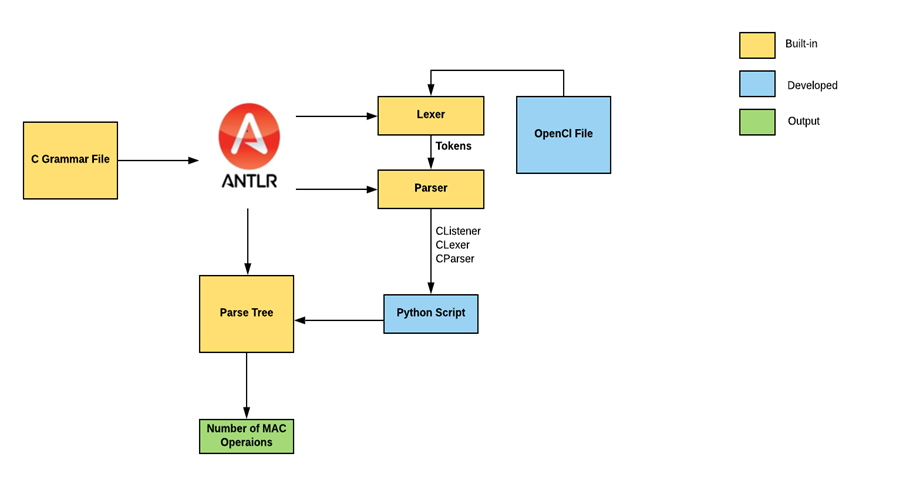
\includegraphics[scale=1.2,width=\textwidth]{img/Antlr4.png}
  \caption{ANTLR4 workflow}
  \label{fig:ANTLR4}
\end{figure}
\pagebreak
\inputminted[breaklines=true]{Python}{img/Antlr4_Python.py}
\captionof{code}{Source Code : OpsCalculator.py\label{code:ANTLR4_Source}}



\begin{code}[!htb]
 \begin{minted}[fontsize=\small]{bash}
[user@fe-1 ~]$ python OpsCalculator.py -kernelfile <path to kernel file> [-v]
\end{minted}
\caption{Command to invoke ANTLR4 based Performance Modeling Tool}
\label{code:ANTLR4Invoke}
\end{code}




\section{Performance Modeling script}
We have used a python script to automate performance modeling for implementations of both GoogLeNet and ResNet. The script considers one kernel at a time, to compute different performance metrics. The metrics are computed according to the specific design of the topology. Thus the given code snippet is for GoogLeNet global memory optimized design and thus needs to be modified for the other designs. The script needs the input and output dimensions of the specific kernel (CNN layer) from the IR along with the execution time from the profiler report in addition to the basic type of kernel such as Conv or Pool. The script is reproduced in Code \ref{code:PerfModel}.

\inputminted[breaklines=true]{Python}{img/PerfModel.py}
\captionof{code}{Source Code : PerformanceModel.py\label{code:PerfModel}}




\section{Python script to generate expected results of CNN Layer}
The functional testing of GoogLeNet and Resnet-50 was carried out by comparing the results at the end of each layer (and/or kernel) with the results generated by TensorFlow running the same models on the same set of inputs. The code used to generate output from TensorFlow has been reproduced in Code \ref{code:TensorFlow}.

\inputminted[breaklines=true]{Python}{img/TensorFlow.py}
\captionof{code}{Source Code : TensorFlow.py\label{code:TensorFlow}}

\section{Python Script to compare Kernel outputs with Tensorflow Outputs}
We can compare the output of our OpenCL implementation with Tensorflow output by using the below code. It generates the Absolute Error between the two outputs.  Python 3 or higher with NumPy 1.16 is necessary to run the code. 

\inputminted[breaklines=true]{Python}{img/abs_error.py}
\captionof{code}{Source Code : abs\_error.py\label{code:abs_error}}

\textbf{Running the script}
For running the script to compare the values, first you should edit the script with file paths and save the script.
\begin{enumerate}
\item Go to line 11 and 13 update the \texttt{tf\_path} and \texttt{tf\_filename} the location to your tensorflow output file.
\item Go to line 16 and 18 update the \texttt{kernel\_path} and \texttt{kernel\_filename} the location to your kernel output file.
\item Run the Python command \\*
          \texttt{python abs\_error.py}
\end{enumerate}

\section{Synthesis Jobs on Notctua Infrastructure}
To execute the CNN topologies the design needed to be synthesized and bitstreams were required to be generated. There are two platform within the $PC^{2}$ infrastructure:
\begin{itemize}
    \item CC- Frontend
    \item Noctua Compute nodes
\end{itemize}
Both of these platforms can be used for synthesizing designs. However, even though the CC-frontend is capable of synthesizing and generating the bitstreams it is not designed for that purpose. For FPGA syntheis there are dedicated compute nodes present in Noctua infrastructure. There are total of 256 compute nodes present which are partitioned into small cluster according to type of synthesis jobs that needs to be carried out.
\newline
For the entirety of the project the compute nodes within \textit{fpgasyn} and \textit{long} partitions were used to generate all the bitstreams.
Noctua cluster uses \raggedright\texttt{Simple Linux Utility for Resource Management (SLURM)} as a workload manager. One has to create a shell script to submit a job to the SLURM workload manager. These are generally called sbatch files. This sheel script contains all the paramaters and the command required to generate a bitstream.
\newpage
\textbf{Batch script for synthesis job}
\begin{minted}{bash}
#!/bin/bash
#SBATCH -N 1
#SBATCH -J unit0
#SBATCH -A hpc-lco-kenter
#SBATCH -p fpgasyn
#SBATCH -t 40:00:00
#SBATCH --mail-type all
#SBATCH --mail-user test@example.com

aoc -v -profile -fp-relaxed -fpc -board=p520_max_sg280l -o /upb/scratch/departments/pc2/groups/pc2-cc-user/custonn2/designs/resnet_units_opv1_bitstream/unit0.aocx unit0.cl -global-ring -duplicate-ring 
\end{minted}
\textbf{Initating a synthesis job}
\begin{enumerate}
    \item Connect to the Noctua Load Balancer using \raggedright\texttt{ssh fe.noctua.pc2.uni-paderborn.de} command
    \item Connect to the compute nodes using \raggedright\texttt{ssh noctua} command
    \item Go the directory where bash script for sbatch is present
    \item Run the sbatch file using \raggedright\texttt{sbatch <filename>.sh} \\*
    \item Type \raggedright\texttt{squeue <username>} to view all the synthesis job
    
\end{enumerate}